\section{Dynamics in an Asymmetric Hamiltonian} \label{sec:asymham}

The previous section, and much of the current literature, focuses on symmetric Hamiltonian systems, in that the butterfly velocity is the same for perturbations traveling to the left or to the right. Ref.\cite{??} mentions...

In this section we study the operator dynamics of an asymmetric time-independent Hamiltonian system. First we construct the local 3-site Hamiltonian through its action on the computational basis. 
After chaining together these local terms to define a multi-site Hamiltonian we find the behavior of the Pauli weights and OTOC. Eventually we show that this system has two distinct butterfly velocities, one for operator fronts spreading in each direction.

\subsection{3-Site Hamiltonian}  \label{sub:hamiltonian}

We want a multi-site in which sites interact only through local interactions. We can accomplish this by defining an $n$-site Hamiltonian for $n$ small, and then putting this Hamiltonian on each set of $n$ sites,
\begin{align}
H_{\text{tot}} = \sum_{i=1}^{L-n}H_n(\psi_i,\psi_{i+1},\dots\psi_{i+n})
 \label{eqn:chain}
\end{align}
A common choice is $n=2$ but this will not suffice, because 2-site Hamiltonians are always symmetric.\footnote{Is this true?} There do exists asymmetric Hamiltonians for three sites, though. 

The feature we are looking for in this Hamiltonian is asymmetry in its dynamics. To that end, instead of looking directly for an asymmetric Hamiltonian, we can find a unitary operator $U(t)$ with the dynamics we want. From that operator we can construct a Hamiltonian that gives $U(t)=e^{-iHt}$. There are multiple ways to construct $H$ from $U(T)$. One way is to just take the matrix log, for example by using Mathematica. Since this method is not very physical, we can instead look at eigenstates. $U(t)$ and $H$ will have the same eigenstates, with the eigenvalues of $H$ given by $\lambda_H = i\log(U(1))$. The Hamiltonian is completely specified by its eigenstates and eigenvalues. Since scalar logs are easier, this method is much more intuitive.

One asymmetric unitary operator is the 3-site swap $S_{123}$. $S_{123}$ is a unitary operator such that\footnote{Notation}
\begin{align}
S_{123}\ket{\psi_1\psi_2\psi_3} =\ket{\psi_3\psi_1\psi_2}, \label{eqn:condition}
\end{align}
where the position of the wavefunction denotes the site on which it sits. The idea of using this operator is that it can transport a state from the left side to the right side in 1 step, but takes two applications to move a state from the right to the left.

One way to build the three site swap gate is in a Floquet system or quantum circuit, out of 2-site swap gates $S_{123} = S_{12}S_{23}$. Each 2-site swap interchanges two states, so the action is 
\begin{align}
S_{12}S_{23}\ket{\psi_1\psi_2\psi_3} &= S_{23}\ket{\psi_1\psi_3\psi_2} = 
	\ket{\psi_3\psi_1\psi_2}\nn
&= S_{123}\ket{\psi_1\psi_2\psi_3}.
\end{align}
It is also possible to build $S_{123}$t out of a time-independent Hamiltonian, so that $U(1) = e^{-iH_3} = S_{123}$. We will construct the Hamiltonian using the eigendecomposition, but it is also possible to take the matrix log.

For a system with spin-$\half$ objects on the sites there is an 8-dimensional Hilbert space, which can be decomposed into a spin-$\frac{3}{2}$ subspace with 4 states and 2 spin-$\half$ subspaces with 2 states each. Since the eigenstates of $S_{123}$ only pick up a phase under unitary evolution, they will be states in which individual particle states differ only by phases, so that the phase from the dynamics effectively permutes the states. 

There are four states that are symmetric with respect to the three sites, and therefore should not change in time and have 0 energy. Before normalization these are
\begin{align}
\ket{\psi_{0,0}}=\ket{000},\quad \ket{\psi_{0,1}}=\ket{100}+\ket{010}+\ket{001},
	\nn
\ket{\psi_{0,3}}=\ket{111},\quad \ket{\psi_{0,2}}=\ket{011}+\ket{101}+\ket{110}.
	\label{eqn:zero}
\end{align}
Of the four other states, two should have positive energy and two should have negative energy. Since $U(3)=1$, their eigenvalues must be cube roots of unity. The energies should be $E_\pm = \pm\frac{2\pi}{3}$ so they pick up a phase $\phi_\pm =e^{-iE_\pm} = e^{\mp i\frac{2\pi}{3}}$. Using condition~\ref{eqn:condition}, we can show that the positive energy states are
\begin{align}
\ket{\psi_{+,1}}=&\ket{100} + \phi_-\ket{010} + \phi_+\ket{001},\nn
\ket{\psi_{+,2}}=&\ket{011} + \phi_-\ket{101} + \phi_+\ket{110},\label{eqn:plus}
\end{align}
while the negative energy states are 
\begin{align}
\ket{\psi_{-,1}}=&\ket{100} + \phi_+\ket{010} + \phi_-\ket{001},\nn
\ket{\psi_{-,2}}=&\ket{011} + \phi_+\ket{101} + \phi_-\ket{110}.\label{eqn:min}
\end{align}
For example. the evolution of $\ket{\psi_{+,1}}$ is
\begin{align}
U(1)\ket{\psi_{+,1}} &= \phi_+ \left(\ket{100} + \phi_-\ket{010} + \phi_+
	\ket{001}\right)\nn
&= \phi_+\ket{100} + \ket{010} +\phi_- \ket{001}\nn
&= S_{123}\ket{\psi_{+,1}},
\end{align}
with similar results for the other 3 non-zero energy states.

To write the Hamiltonian as a matrix we have to choose a basis. In the eigenbasis, of course, the Hamiltonian is diagonal. A more useful basis is the computational basis, which has states $\ket{000},\,\ket{001},\,\ket{010},$ etc,
Then the Hamiltonian is 
\begin{align}
H_3 = T\; \text{diag}(0,0,0,0,E_+,E_+,E_-,E_-)\; T^\dag,
\end{align}
where diag(\dots) is the Hamiltonian in its eigenbasis and $T$ is the transformation matrix between the two bases, which can be found from the form of the 3 eigenstates in Eqs.~\ref{eqn:zero}, \ref{eqn:plus}, and~\ref{eqn:min},
\begin{align}
T = \th{\sqrt{3}}\begin{bmatrix}
\sqrt{3} & 0 & 0 & 0        & 0      & 0      & 0      & 0      \\
0        & 1 & 0 & 0        & \phi_+ & 0      & \phi_- & 0      \\
0        & 1 & 0 & 0        & \phi_- & 0      & \phi_+ & 0      \\
0        & 0 & 1 & 0        & 0      & 1      & 0      & 1      \\
0        & 1 & 0 & 0        & 1      & 0      & 1      & 0      \\
0        & 0 & 1 & 0        & 0      & \phi_- & 0      & \phi_+ \\
0        & 0 & 1 & 0        & 0      & \phi_+ & 0      & \phi_- \\
0        & 0 & 0 & \sqrt{3} & 0      & 0      & 0      & 0
\end{bmatrix}
\end{align}
Altogether, the Hamiltonian is
\begin{align}
H_3 = \frac{2\pi i}{\sqrt{3}}\begin{bmatrix}
0 & 0  & 0  & 0  & 0  & 0  & 0  & 0 \\
0 & 0  & 1  & 0  & -1 & 0  & 0  & 0 \\
0 & -1 & 0  & 0  & 1  & 0  & 0  & 0 \\
0 & 0  & 0  & 0  & 0  & -1 & 1  & 0 \\
0 & 1  & -1 & 0  & 0  & 0  & 0  & 0 \\
0 & 0  & 0  & 1  & 0  & 0  & -1 & 0 \\
0 & 0  & 0  & -1 & 0  & 1  & 0  & 0 \\
0 & 0  & 0  & 0  & 0  & 0  & 0  & 0 \\
\end{bmatrix}\label{eqn:3ham}
\end{align}
Before moving on we note that this commutes with the total spin-Z operator 
\begin{align}
S_Z = \text{diag}(\frac{3}{2}, \frac{1}{2}, \frac{1}{2}, -\frac{1}{2}, \frac{1}{2}, -\frac{1}{2}, -\frac{1}{2}, -\frac{3}{2})
\end{align}
so total spin-Z is conserved. It also commutes with the other components of spin and therefore also total spin $S^2$.

There are a few checks we can perform on this Hamiltonian, First,it should be symmetric under a simultaneous rotation of all three spins in real space, so that it can be written as $H_3(\bm{\sigma}_1,\,\bm{\sigma}_2 ,\,\bm{\sigma}_3)$. Furthermore it should be antisymmetric under the interchange of any two spins (equivalent to reversing the direction of propagation). The only function of three vectors that has this property is the triple product $H_3= \bm{\sigma}_1\cdot\left(\bm{\sigma}_2 \times\bm{\sigma}_3\right)$, where multiplication of components is interpreted as tensor products.

The representation of the Hamiltonian as a triple product provides another reason for the spectrum of the Hamiltonian. As previously mentioned the Hilbert space of the 3 spins decomposes into one spin-$\frac{3}{2}$ space and two spin-$\half$ spaces. The state $\ket{111}$ is part of the spin-$\frac{3}{2}$ space. Since the three spins point in the same direction, their triple product vanished. Furthermore, since the other three states in the spin-$\frac{3}{2}$ subspace are related to $\ket{111}$ by rotation and the Hamiltonian is symmetric in this respect they also must have energy 0. Of the two spin-$\half$ pairs, one pair has positive energy and one has negative energy.

%This triple product is
%\begin{align}
%H &= \bm{\sigma}_1\cdot\left(\bm{\sigma}_2 \times\bm{\sigma}_3\right) \nn
% &= \sigma_{1,1}\otimes\sigma_{2,2}\otimes{\sigma}_{3,3} - {\sigma}_{1,1}
%	\otimes\sigma_{2,3}\otimes\sigma_{3,2} + \sigma_{1,2}\otimes{\sigma}_{2,3} \otimes {\sigma}_{3,1}-\cdots
%\end{align}
%which is indeed equivalent to Eq.~\ref{eqn:3ham}.

Exponentiating the Hamiltonian should act as another check. This gives the time evolution operator for one time step
\begin{align}
U(1) = e^{-iH_3} = \begin{bmatrix}
1 & 0 & 0 & 0 & 0 & 0 & 0 & 0 \\
0 & 0 & 1 & 0 & 0 & 0 & 0 & 0 \\
0 & 0 & 0 & 0 & 1 & 0 & 0 & 0 \\
0 & 0 & 0 & 0 & 0 & 0 & 1 & 0 \\
0 & 1 & 0 & 0 & 0 & 0 & 0 & 0 \\
0 & 0 & 0 & 1 & 0 & 0 & 0 & 0 \\
0 & 0 & 0 & 0 & 0 & 1 & 0 & 0 \\
0 & 0 & 0 & 0 & 0 & 0 & 0 & 1
\end{bmatrix}
\end{align}
This has the properties of of condition~\ref{eqn:condition}. Furthermore, application three times gives $U(3) = 1$. 

We can learn more about this Hamiltonian by watching the evolution of a single state. If the system starts in the state $\ket{100}$, the coefficients for the other states with equal total $S_Z$ will both change from 0 while the other coefficients will stay 0 due to conservation of $S_Z$.
The state will become $\ket{010}$ at time 1. Fig.~\ref{fig:timeevol} shows this evolution. An important point to realize is that the coefficient of $\ket{001}$ also becomes non-zero at early time, as it must for evolution under a time-independent Hamiltonian if it is going to become non-zero in the future. 
\begin{figure}
	\centering
	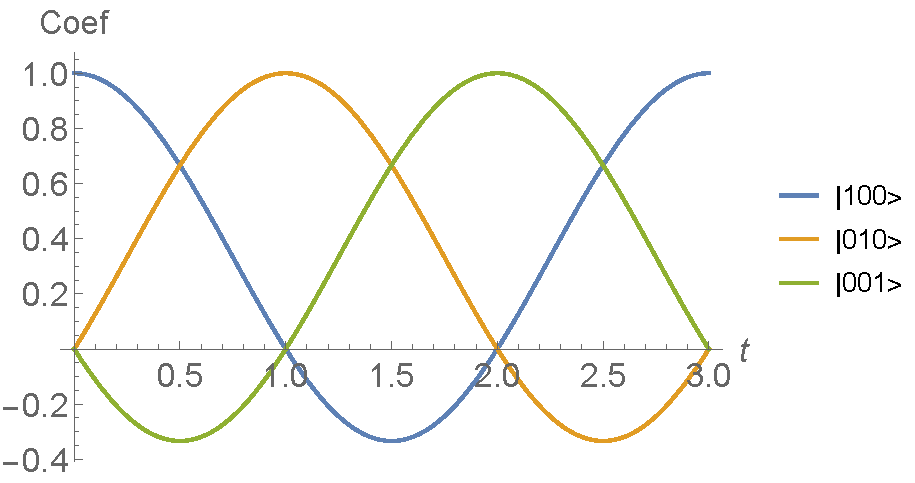
\includegraphics[width=.5\textwidth]{timeevol}
	\caption{Evolution of coefficients if the system starts in state $\ket{100}$.}
	\label{fig:timeevol}
\end{figure}

\subsection{Multi-Site Hamiltonian} \label{sub:multistate}

The 3-site system is periodic, and furthermore is not large enough to effectively study operator spreading. One way would be to apply $H_3$ repeatedly to each triplet of spins. This would equivalently apply $S_{123}$ to each triplet. However this is not a time-independent Hamiltonian, but rather a Floquet system. To preserve time independence we can apply the 3-site Hamiltonian to all triplets simultaneously, as in Eqn.~\ref{eqn:chain}. Note that this means that $U(t)$ will no longer have a simple form like Eqn.~\ref{eqn:condition}. This subsection will explore the dynamics of this multi-site Hamiltonian.

\subsubsection{Construction} \label{subsub:construction} 

Explicitly, the extension of this Hamiltonian to 4 sites is
\begin{align}
H_4 = H_5\otimes\mathbb{I} + \mathbb{I}\otimes H_3.
\end{align}
This Hamiltonian still preserves each component of total spin. Since we are applying the Hamiltonian to the 4 sites simultaneous, its unitary behavior does not simply swap states between the sites. However, the behavior is still periodic. Fig.~\ref{fig:timeevol4} shows that when the system starts in state $\ket{0001}$ it returns to that state with period $\tau=3\sqrt{\frac{3}{5}}$ but never fully reaches any other basis state.
\begin{figure}
\centering
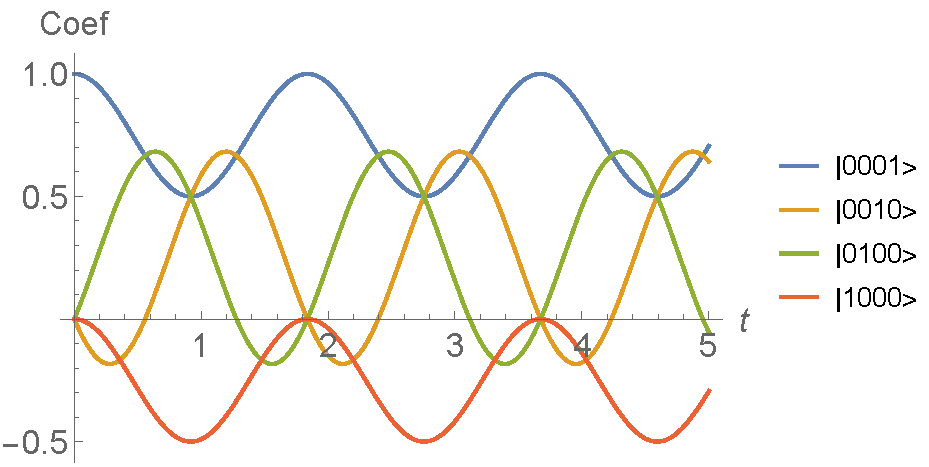
\includegraphics[width=.5\linewidth]{timeevol4}
\caption{\textbf{Evolution of the 4-site system} when the initial state is $\ket{0001}$. Each curve is the coefficient of one of the basis states. The system is periodic with period $\tau=3\sqrt{\frac{3}{5}}$, and is never fully in one of the other basis states.}
\label{fig:timeevol4}
\end{figure}

With 5 sites, adding the third triplet destroys the simple periodic behavior of the system. The Hamiltonian is now
\begin{align}
H_5 = H_3\otimes\mathbb{I}_2 + \mathbb{I}\otimes H_3\otimes\mathbb{I} +
	\mathbb{I}_2\otimes H_3.
\end{align} 
Starting in $\ket{00001}$, the coefficients follow the pattern of figure~\ref{fig:timeevol5}. At first the evolution is similar to the $n=1$ case, with $\ket{10000}$ and then $\ket{01000}$ reaching near maximal. This suggests that the system retains some of its swap gate-like behavior. However the system is never fully in any basis state after $t=0$, due to the lack of periodicity.

By directly diagonalizing the Hamiltonian we can study the evolution of a single component of the state. The coefficient of $\ket{00001}$ is 
\begin{align}
c_1(t) = \frac{1}{10} \left(3 \cos \left(\frac{2}{3} \sqrt{\frac{5}{3}} \pi  t\right)+5 \cos \left(\frac{2 \pi  t}{3 \sqrt{3}}\right)+2\right)
\end{align} 
which is shown in figure~\ref{fig:onecoef}. Although it appears to be quasi-periodic, it cannot ever reach 1 for $t\ne 0$ or be truly periodic because its the periods of the two cosine functions are not rationally related.

\begin{figure}
	\centering
	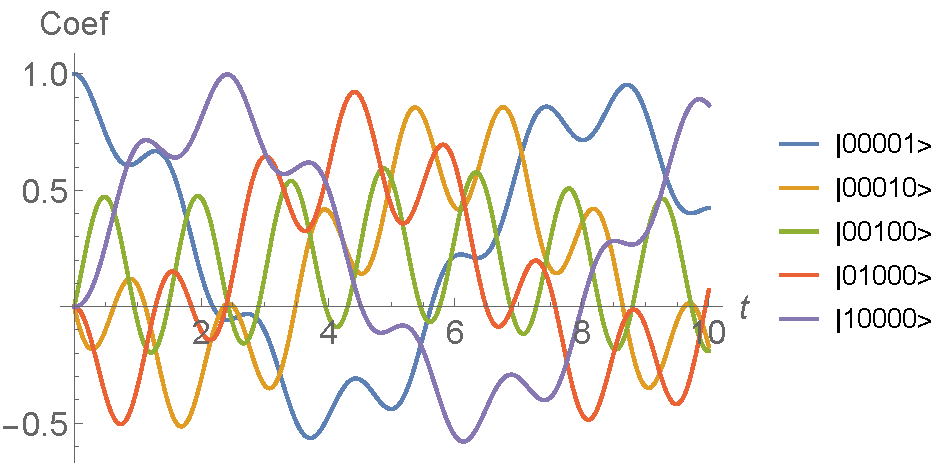
\includegraphics[width=.6\textwidth]{timeevol5dense}
	\caption{\textbf{Evolution of the 5 site system} when the system starts in state $\ket{00001}$. Periodicity is ruined by the third triplet.}
	\label{fig:timeevol5}
\end{figure}

\begin{figure}
	\centering
	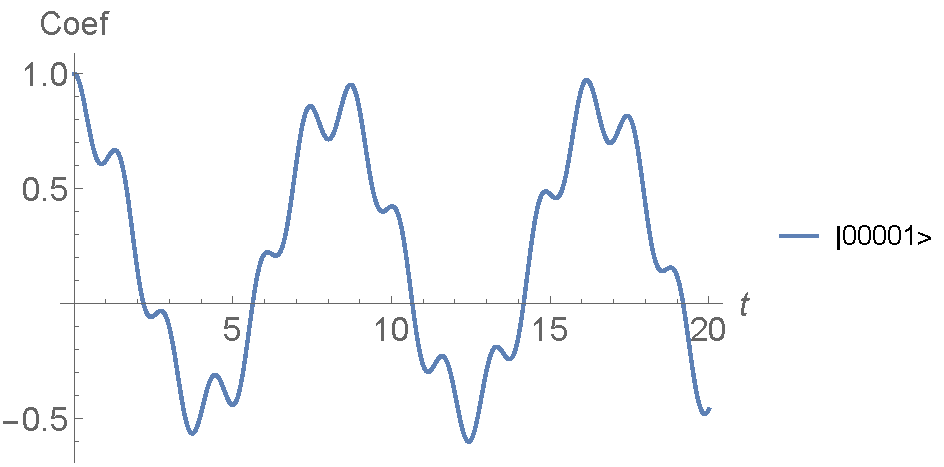
\includegraphics[width=.5\textwidth]{onecoefd}
	\caption{\textbf{Simplified view of Fig.~\ref{fig:timeevol5}}, showing only the coefficient for $\ket{00001}$ when that is the starting state. Even with the longer range of time, the coefficient never returns to 1.}
	\label{fig:onecoef}
\end{figure}

%The coefficient for $\ket{00100}$ does not fit the pattern. It does not reach maximum at the right time and it does have a periodic structure. Furthermore, when the starting state is $\ket{00010}$ the problematic state is still $\ket{00100}$, probably because of the chaining mechanism. When the starting state is $\ket{00100}$ the coefficients for $\ket{10000}$ and $\ket{00001}$ always vanish. The next chaining method to try will be to have $2n$ spins, and to have the first spin complete the last trio.

Instead of putting $H_3$ on every triplet, we can only chain together the odd triplets. We will call these sparse systems, and they are only possible for odd $L$. For example the sparse Hamiltonian for $L=5$ is
\begin{align}
H'_5 = H_3\otimes\mathbb{I}_2 + \mathbb{I}_2\otimes H_3.
\end{align}
Like the dense $L=5$ Hamiltonian, this system is not periodic. A plot of the coefficients over time the the starting state $\ket{00001}$ is shown in Fig.~\ref{fig:timeevol5s}. An interesting detail is that the coefficient on state $\ket{00100}$ is actually periodic. 
\begin{figure}
	\centering
	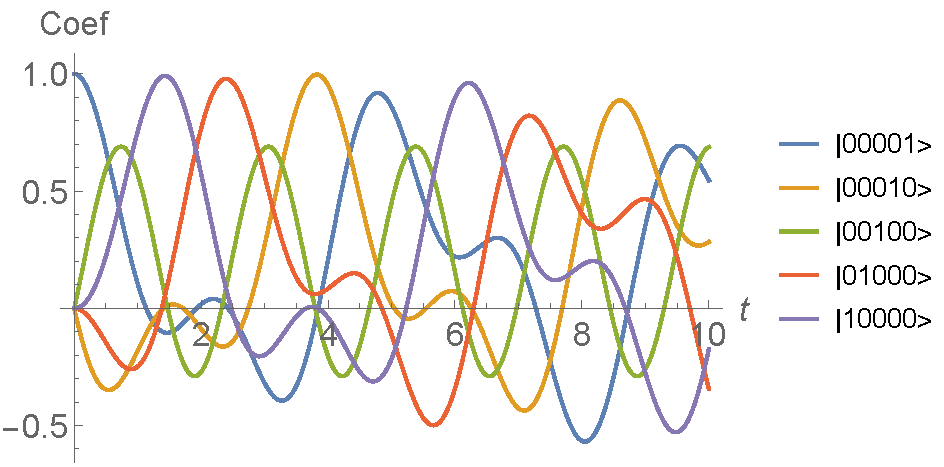
\includegraphics[width=.5\linewidth]{timeevol5}
	\caption{\textbf{Evolution of the sparse 5-site system}. Although the coefficients for most states are not periodic, the coefficient for $\ket{00100}$ is.}
\end{figure} 
This is the last vestige of periodicity left over from the small systems, and provides a small argument for using the dense systems, since the aperiodic systems spread more fully.

Note that the previous analysis has focused only on individual states, not operator spreading. Furthermore, for larger systems, looking at all coefficients becomes unwieldy. We can solve these problems simultaneously by using the tools developed in the previous section for quantifying operator spreading.

\subsubsection{Pauli String Weight} \label{subsub:pauli}  

We can study the operator dynamics of this system by extending to large $L$ and evolving operators that are identities on all sites except one end. Since the Hamiltonian is SO(3) symmetric, it does not matter if the perturbation is $X$, $Y$, or $Z$. For convenience, we will use $Z$. We start by discussing the Pauli weight, and delay discussing the OTOC and butterfly velocity to Sec.~\ref{subsub:otoc}.

The first Hamiltonian we will discuss is the $L=11$ sparse Hamiltonian.
For the forward-propagating wave, with $A(t=0) = Z_0 = Z\otimes \mathbb{I} \otimes \mathbb{I} \cdots$, the weight all starts on site 0. As it evolves, it reaches peaks for even sites, but does not rise above $1/10$ for the odd sites. The successive peaks fall off in size but dominate the Pauli strings until the last site takes over. This evolution can be seen in Fig.~\ref{fig:L11end3n20front}). 

To understand this behavior, realize that 

For the backward-propagating waves $(A(t=0)=Z_{L-1})$, the initial decaying signal is more difficult to make out but still present. It is dominated by a large weight of sites that start on site 9 around $t=1$. By $t = 3$ the first site has started to dominate the Pauli weights.

\begin{figure}
	\centering
	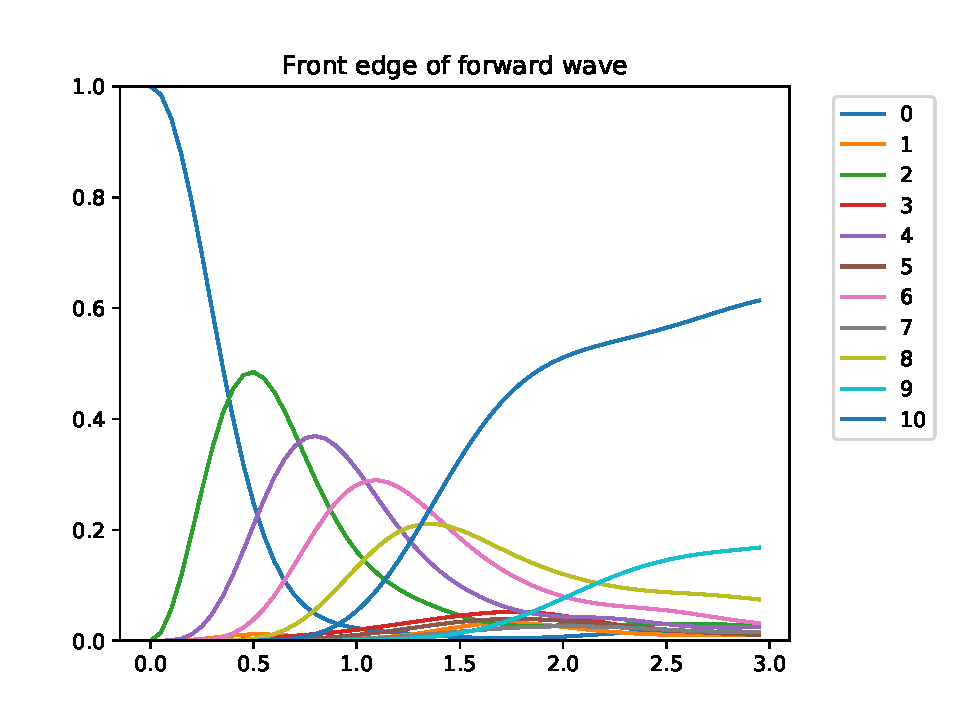
\includegraphics[width=.7\textwidth]{L11end3n20front}
	\caption{Weight of operators that end on site $i$.}
	\label{fig:L11end3n20front}
\end{figure}
\begin{figure}
	\centering
	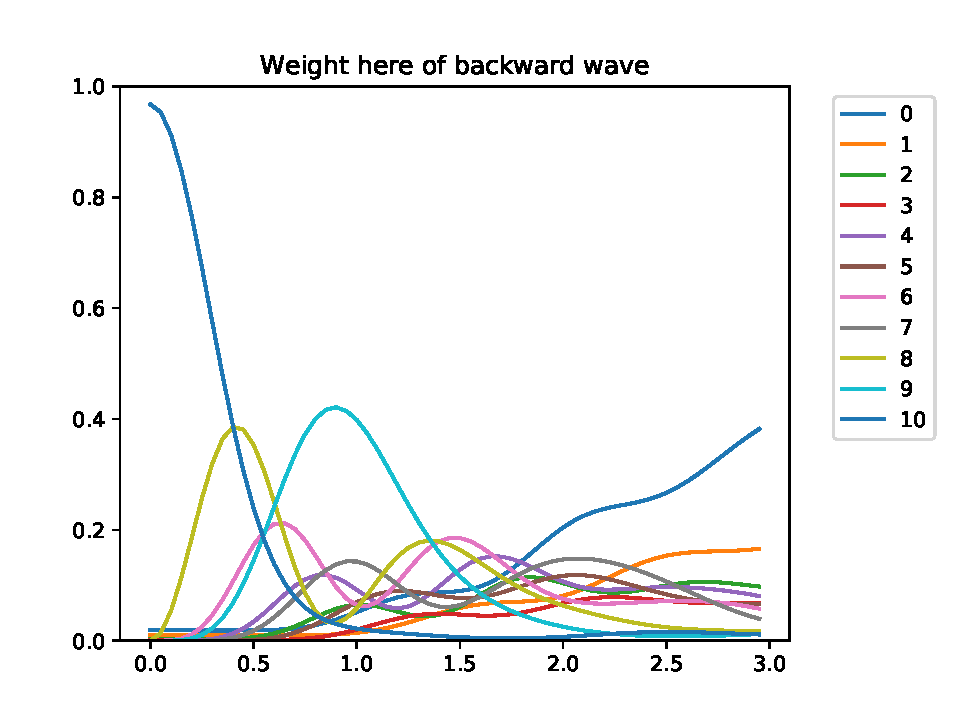
\includegraphics[width=.7\textwidth]{L11end3n20back}
	\caption{Weight of operators that begin on site $i$.}
	\label{fig:L11end3n20back}
\end{figure}

The initial behavior also matches the $L=9$ case. For forward propagation the initial behavior is $W(t;i) = ae^{bt}$ with $a,b$ given by\dots Figure~\ref{fig:L11end1n60fore} shows this behavior, while figure~\ref{fig:L11end1n60back} shows the analogous behavior for the backward propagating wave. 

\begin{figure}
	\centering
	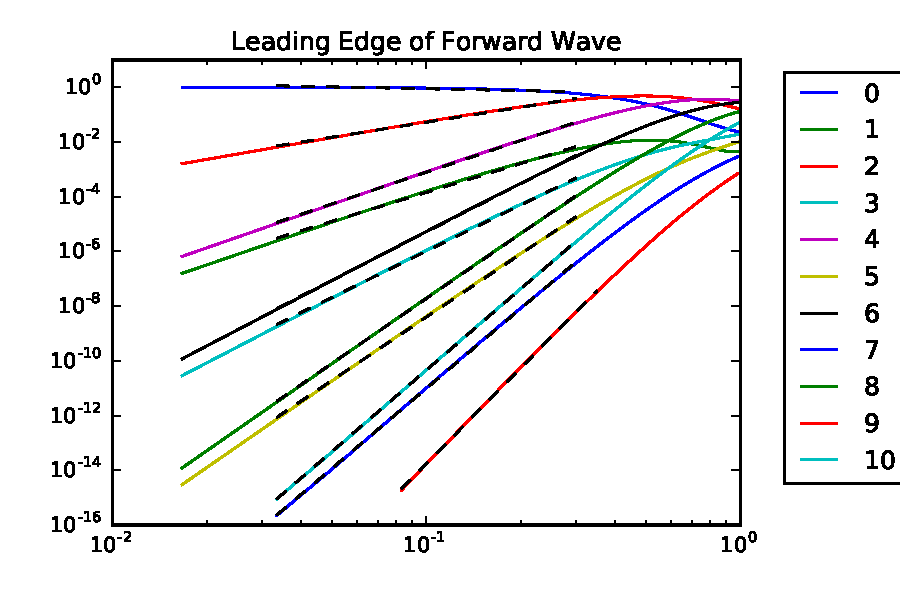
\includegraphics[width=.7\textwidth]{L11end1n60fore}
	\caption{Early-time leading edge weights for forward propagating wave.}
	\label{fig:L11end1n60fore}
\end{figure}
\begin{figure}
	\centering
	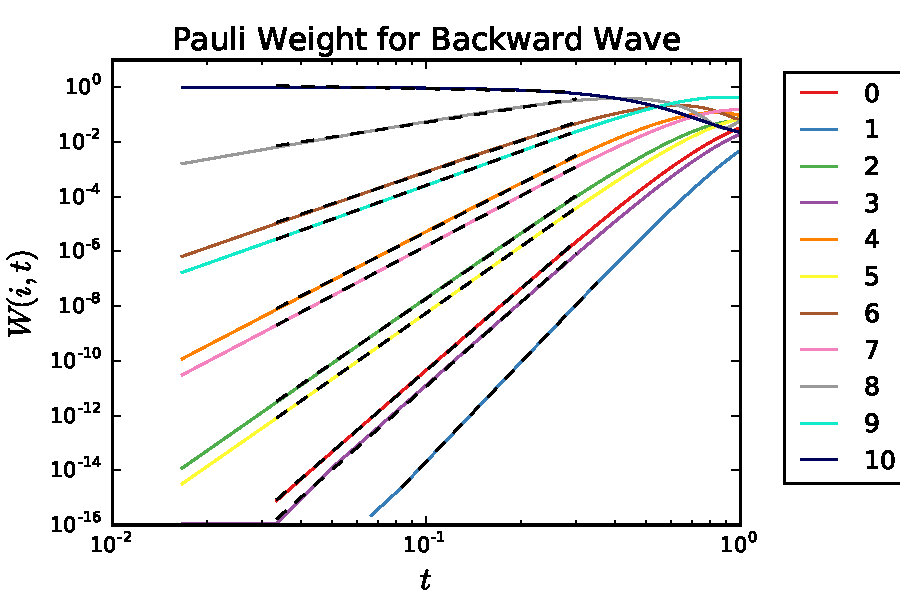
\includegraphics[width=.7\textwidth]{L11end1n60back}
	\caption{Early-time leading edge weights for backward propagating wave.}
	\label{fig:L11end1n60back}
\end{figure}

Here the relevant numbers are\dots
Again, the exponents for even and odd sites increase by one within each group. Pairs of sites separated by 3 are also divergent in the forward case while convergent in the backward case.

\subsubsection{OTOC and Butterfly Velocity} \label{subsub:otoc}

After discussing the behavior of the Pauli weights in the sparse and dense Hamiltonians, we will discuss the OTOC, which encodes the amount of operator weight on a site, and from this explore the butterfly velocity. We do not find an explicit $v_B$ but do show that it is different in the two directions.